 \documentclass[amsmath,preprintnumbers,10pt,nofootinbib,prl,twocolumn]{revtex4-1}
\usepackage{amsbsy}
\usepackage{amsmath}
\usepackage{amssymb}
\usepackage{graphicx}
\usepackage{color}
\usepackage{subfig}
\usepackage{physics}
\usepackage{soul}
\usepackage{color}
\usepackage{bm}
\usepackage[normalem]{ulem}

%\newcommand{\Tr}{\text{Tr}}
\newcommand{\Ai}{\text{Ai}}
\newcommand{\Bi}{\text{Bi}}
\newcommand{\Real}{\text{Re}}
\newcommand{\Imag}{\text{Im}}

\usepackage{verbatim}
\usepackage{natbib}
\bibliographystyle{apsrev4-1}
\begin{document}
\title{Supplementary Information: Dissipation induced transitions in elastic strings.}
\author{Michael Nguyen$^{1,2}$, Suriyanarayanan Vaikuntanathan$^{1,2}$} 
\affiliation{$^1$The James Franck Institute, The University of Chicago, Chicago, IL,}
\affiliation{$^2$ Department of Chemistry, The University of Chicago, Chicago, IL.}
\maketitle
\section{Dynamics of the Simulation}
Fig \ref{fig:GrowthRate} and Fig \ref{fig:Variance} show that the growth rate and size variance of the system does not scale linear with t but with its square root. Time here is the number of attempt we add and remove a random particle. This is because in the simulation we only allow addition and remove moves. Thus, the system can only relax through the moves also. Therefore, it will take the system around N*addition/remove steps to relax it to steady state. If we then redefine time, $dt\text{*} = dt/N$ to take into account that many particles can act at same time, then in this new define time t*, our growth rate and size variance will scale linear with time. Using this procedure, we can then extract the growht rate and its variance. Still, this shows that the assembly growth rate does not increase with system size.

\section{Extracting v/D}
In general, the formula for the size of the assembly has the form :
\begin{equation}
 \langle\Delta N\rangle=a\sqrt{t+b}+c
\end{equation}
Here, N is the number of partcile, a is the growth rate, b depends on how one change the origin of time measurement and c is there to captures the effects of other factors such as initial condition and finite size effect. Similarly, the formula for the variance of the assembly when we allow the assembly to grow from the same initial condition is:
\begin{equation}
\langle\delta N^2\rangle =d\sqrt{t+b}+e
\end{equation}
Idealy, one can use the procedure from the previous section to transform $\langle\Delta N\rangle$ and $\langle\delta N^2\rangle$ to a line and extract its rate from there.
Specifically, the procedure will give the slopes:
\begin{equation}
\frac{d\langle\Delta N \rangle}{dt^{*}}=\frac{a^2}{2}+\frac{c}{2\sqrt{t+b}}
\end{equation}
\begin{equation}
\frac{d\langle\delta N^2 \rangle}{dt^{*}}=\frac{ad}{2}+\frac{c}{2\sqrt{t+b}}
\end{equation}
So for a good extraction of a, we would want:
\begin{equation}
\begin{split}
\frac{|c|}{2\sqrt{t+b}}<<\frac{a^2}{2}
\\ t >>\frac{c^2}{a^4}-b
\end{split}
\end{equation}
Thus, depending on the magnitude of a,b,d and c, it might take a long time for them to settle into a line to extract the growing rate of the assembly and its deviation. Specifically, using the values of a,b and c extracted in our current simulation, the time t required will be in the order of $10^{12}$ Monte Carlo steps. 
If we simply want the ratio of a and d for the bound, we can just plot $\langle\Delta N\rangle$ with $\langle\delta N^2 \rangle$ which will give:
\begin{equation}
\langle\Delta N\rangle=\frac{a}{d}\langle\delta N^2 \rangle-\frac{ae}{d}+c
\end{equation}
\begin{figure}[tbb]
\centering
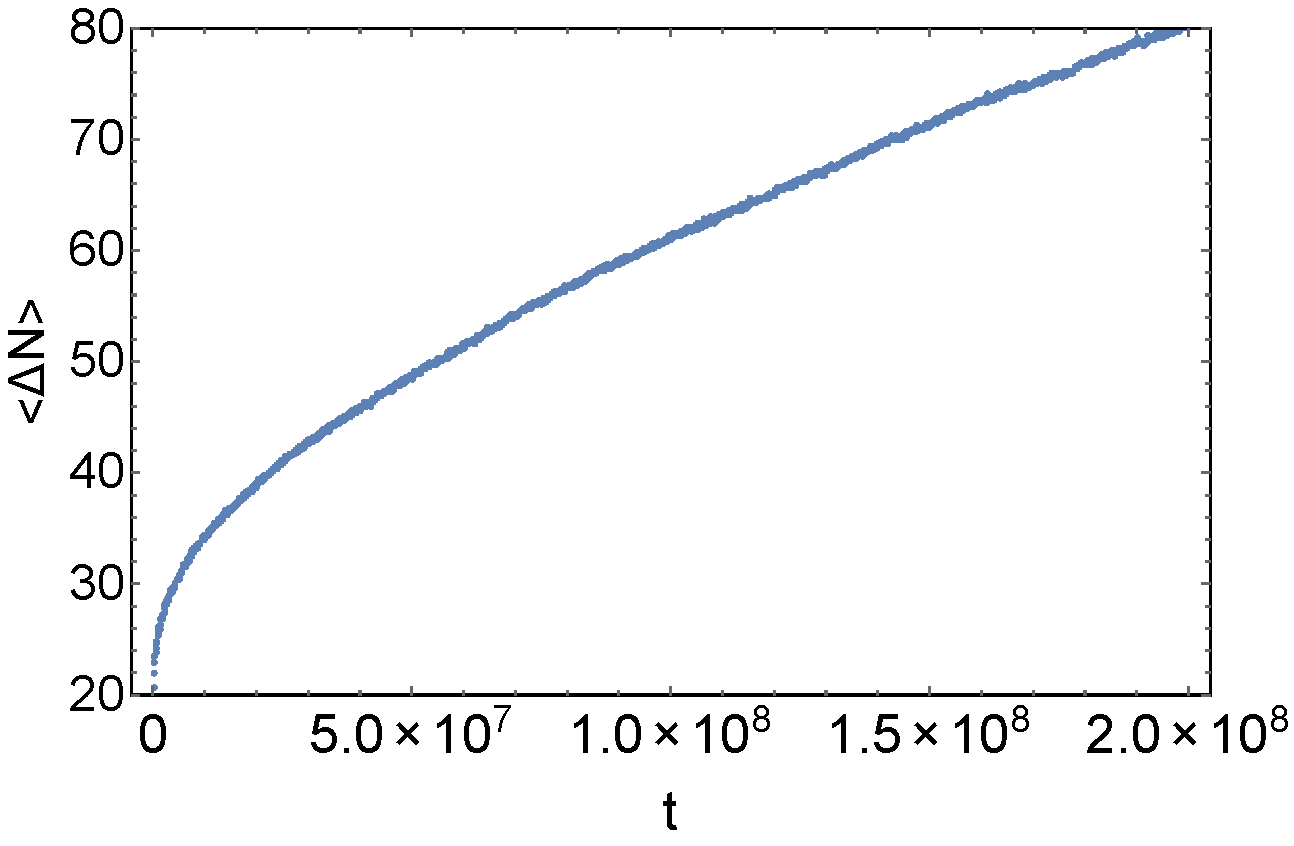
\includegraphics[scale=0.37]{meanofmu3d3k4ktheta6.pdf}
\caption{$\langle\Delta N\rangle$ vs. $t$. The growth rate here is for $\delta \mu = 1.0$ with $k_s=4$ and $k_\theta = 6$.} \label{fig:GrowthRate}
\end{figure}
\begin{figure}[tbb]
\centering
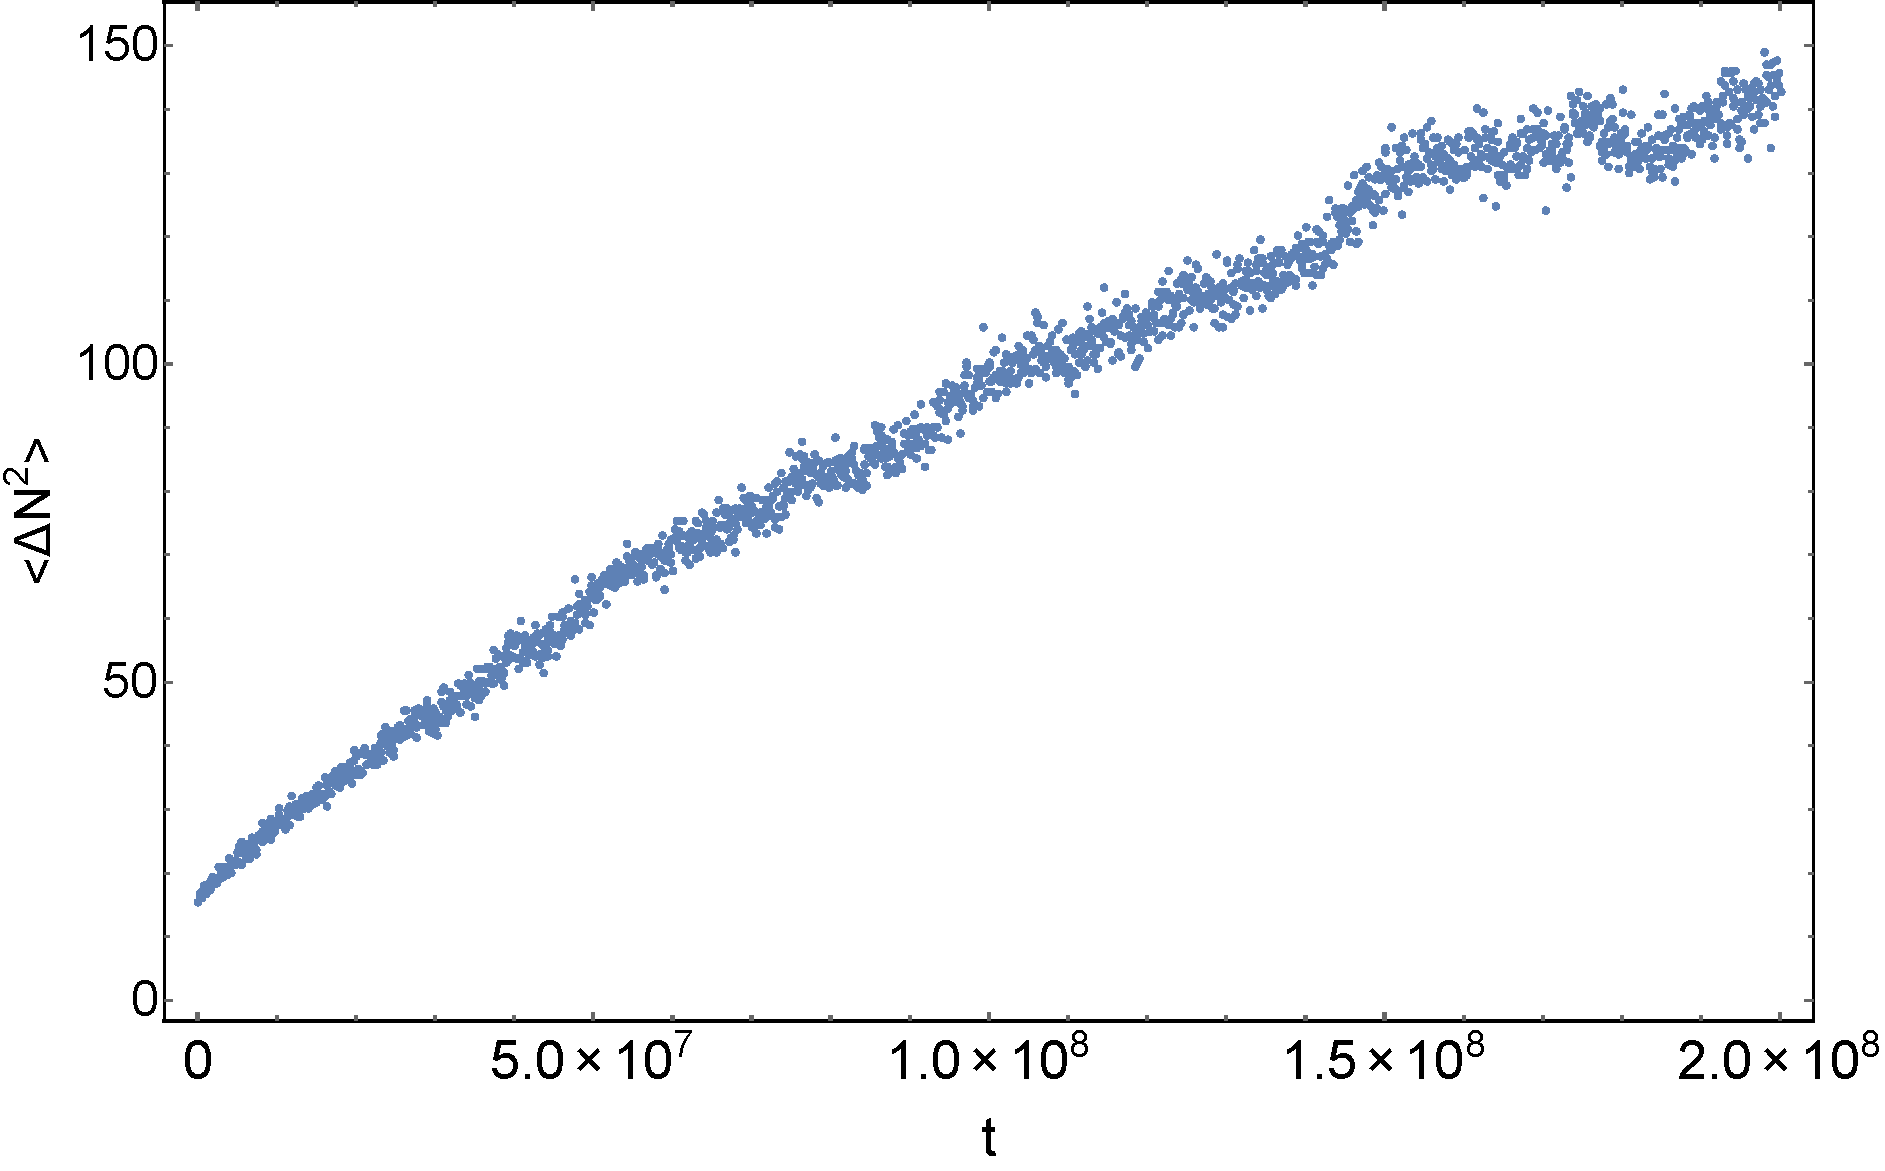
\includegraphics[scale=0.25]{varianceofmu3d3k4ktheta6.pdf}
\caption{$\langle\Delta N^2\rangle$ vs. $t$.The variance here is for $\delta \mu = 1.0$ with $k_s=4$ and $k_\theta = 6$.} \label{fig:Variance}
\end{figure}
\begin{figure}
\centering
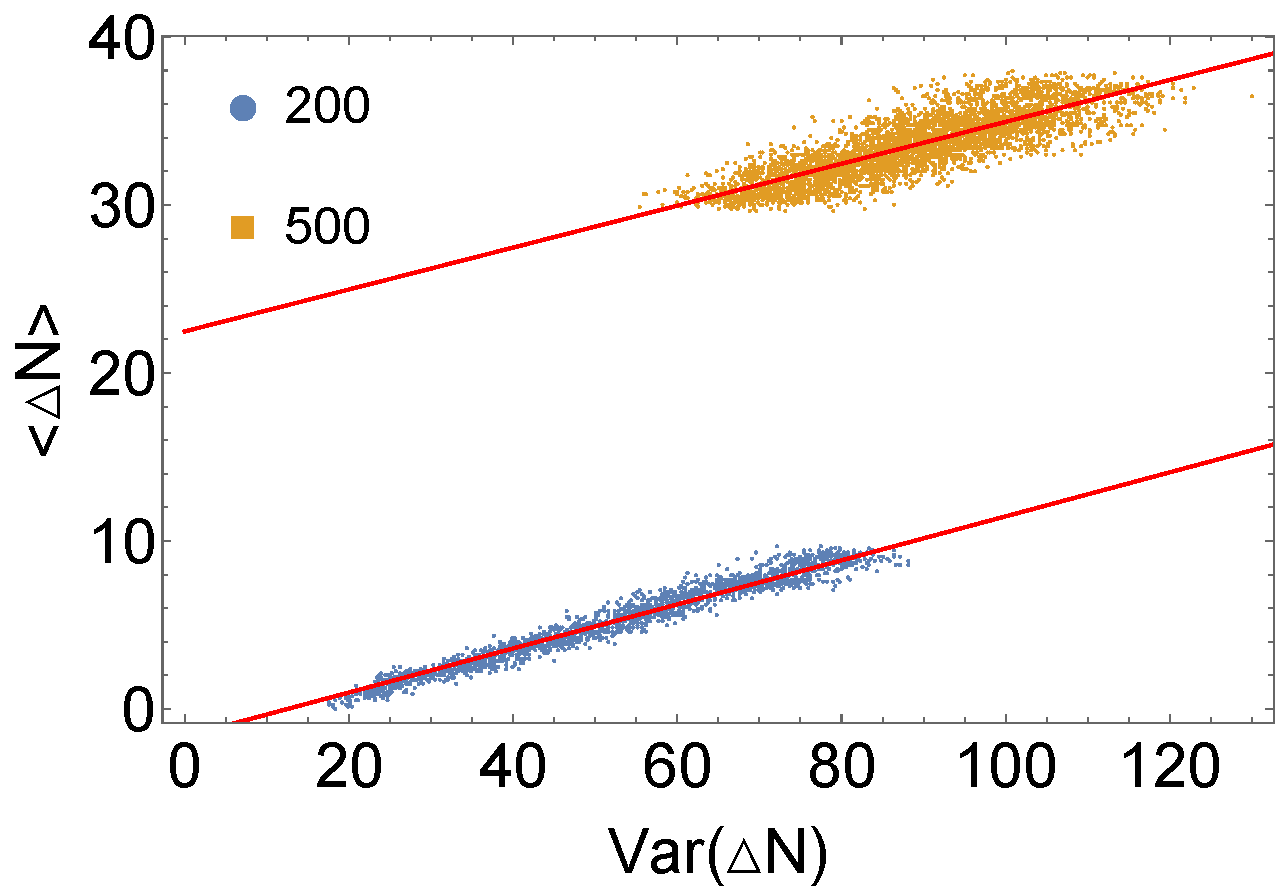
\includegraphics[scale=0.35]{deltaNvsVar.pdf}
\caption{$\Delta N$ vs. $Var(\Delta N)$. The slope extracted here is 0.12 making $\frac{v}{D}=0.24$. The data here is for $\delta\mu=0.26$, $k_s=4$ and $k_\theta = 6$.} \label{fig:fittingvelocity}
\end{figure}
\section{The Simulation}
Here we will describe the algorithms of the simulation. The initial configuration of the assembly is a circle consisting of $N_0$ particles with equal distance between them. Next we will add or remove a particle with equal probability. If the move is addition, first we will choose a random particle in the assembly. We will then draw an arc whose center is the same as the one in the assembly. The arc will span from the previous random particle to the one that is next to it clockwise. In the area spanned by this arc, we will choose the position of the new particle to be added. In the simulation, we keep the area of the arc constant. Then we will accept the move with acceptance rate $\rm{Min}(\rm{Exp}[-\Delta E +\mu],1)$. If the move is removal, we will simply remove a random particle from the assembly with acceptance rate $\rm{Min}(\rm{Exp}[-\Delta E -\mu],1)$. The transition rates of the simulations are:
\begin{equation}
W^{N,N+1}_{ij}=P_i(\bold{l},\bold{\theta})\frac{1}{AN}\rm{Min(Exp[-(E_j - E_i)+\mu],1)}
\end{equation}
\begin{equation}
W^{N+1,N}_{ij}=P_j(\bold{l},\bold{\theta})\frac{1}{N+1}\rm{Min(Exp[-(E_i - E_j)-\mu],1)}
\end{equation}

Fig. ~\ref{fig:SimulationSchematic} shows the schematic of the simulation.
\begin{figure*}[t]
\includegraphics[width=1\linewidth,angle=0]{AddingMoveSchematic.pdf}
\caption{ Schematic of the simulation's addition and remove moves. The addition rate is $W_{ij}^{N,N+1}=\frac{1}{NA} P_i(l_1,l_2,...,l_N,\theta_1,\theta_2,...,\theta_N)\rm{Min}(\rm{Exp}[-(E_j-E_i) +\mu,1])$. The removal rate is $W_{ij}^{N+1,N}=\frac{1}{N+1}P_j(l_1,l_2,...,l_N,l_{N+1},\theta_1,\theta_2,...,\theta_N,\theta_{N+1})\rm{Min}(\rm{Exp}[-(E_i-E_j) -\mu],1)$. Here, A is the area of the arc which we keep constant $A=4$, N is the number of particle in the assembly, $E_j = \frac{k_s}{2}(l_{BE}-l_0)^2+\frac{k_s}{2}(l_{CE}-l_0)^2+k_\theta(\widehat{ABE}-\pi)^2+k_\theta(\widehat{ABE}-\pi)^2+k_\theta(\widehat{ECD}-\pi)^2+C$ and $E_i=\frac{k_s}{2}(l_{BC}-l_0)^2+k_\theta(\widehat{ABC}-\pi)^2+k_\theta(\widehat{BCD}-\pi)^2+C$; C is the energy contribution of the other angles and strings }
\label{fig:SimulationSchematic}
\end{figure*}

\section{Small n modes deviation}
The smallest n modes show some deviation from the Helfrich description as shown in the Fig.~\ref{fig:fit} . The deviation seems to be an apparent increase in the surface tension. This effect might be because the number of the particle $N$ in this simulations is always changing. Thus this might make difficult for the longest wavelength move to relax. In this paper, we have reported the $\gamma$ extracted from the bigger n modes. 
\begin{figure}[tbb]
\centering
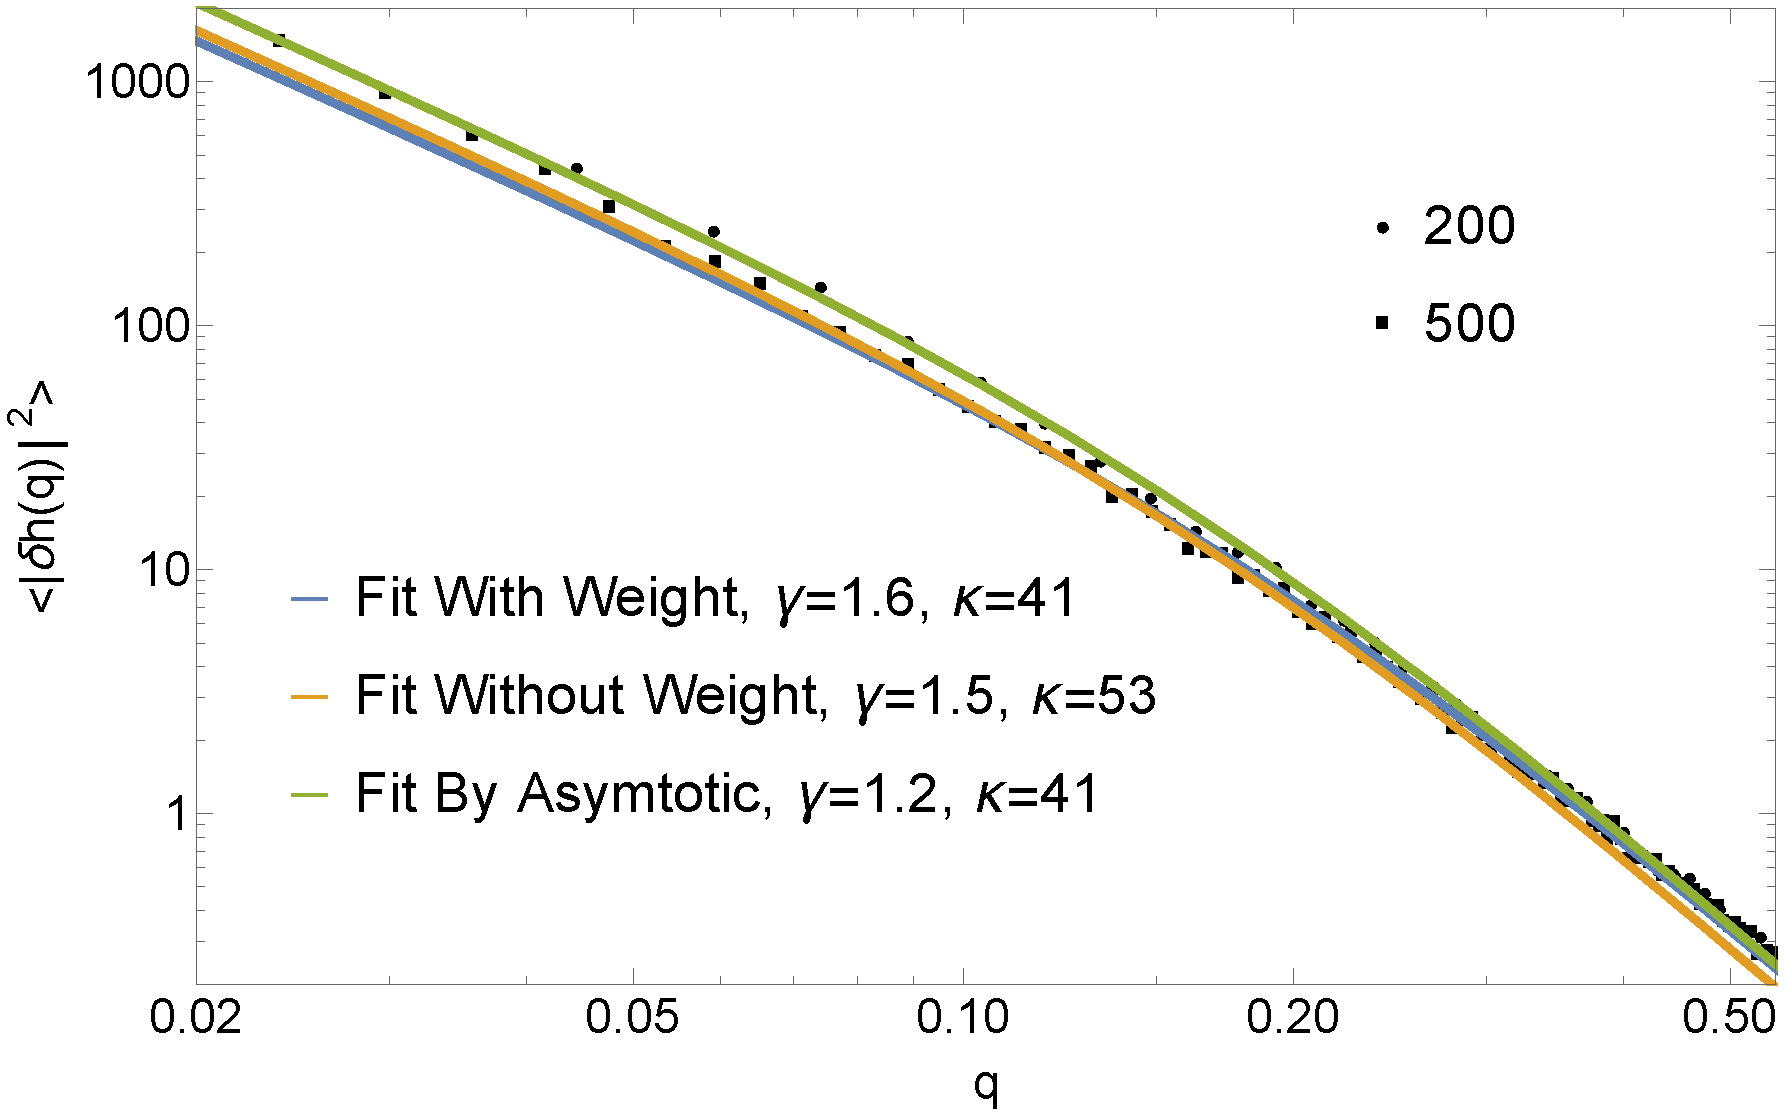
\includegraphics[scale=0.30]{fittingandsmallneffect.pdf}
\caption{$\langle|\delta h(q)|^2\rangle$ vs. $q$ for $\delta \mu \approx 0$ with $k_s=4$ and $k_\theta = 6$. For the smallest n modes, both the 200 and 500 particles spectrums converge to the $\gamma=1.2$ while the rest of the n modes follow $\gamma=1.6$ } \label{fig:fit}
\end{figure}
\section{Fitting Procedure}
In order to extract $\gamma$ and $\kappa$ we need to fit $\langle|\delta h(q)|^2\rangle$ to $\frac{1}{\gamma q^2 +\kappa q^4}$. However, to fit the function correctly, we have to take into account that the variance of the spectrum is not constant. Specifically, the standard deviation of this spectrum is equal to its average. In order words, the errors in measuring in amplitude of the long wavelength modes will be significantly higher than the errors in measuring the amplitudes of the short wavelength ones. This is because each mode can be independently described with an exponential distribution. To fit the spectrum, we have to adjust the weight of the variances in the fitting procedure: $\rm{Weight(q)} = \frac{1}{\rm{Var(\langle|\delta h|\rangle ^2)}}$ so that we do not overfit the long wavelength region.

\section{Predicting Interface Fluctuation}

In the main text, we have used the bounds to predict the required $\delta \mu$ to attain certain effective tension, $\gamma_{\textrm{eff}}$. In a different way, we can use the bounds to predict how increasing $\delta \mu$ affect the surface tension. Fig~\ref{fig:epsilonpredict} shows how Eq. 7 and Eq. 8 in the main text, can be used to predict $\gamma_{\textrm{eff}}$. From the predicted $\gamma_{\textrm{eff}}$, we can construct an effective fluctuation of the interface when it is out of equilibrium. 
\begin{figure}[tbb]
\centering
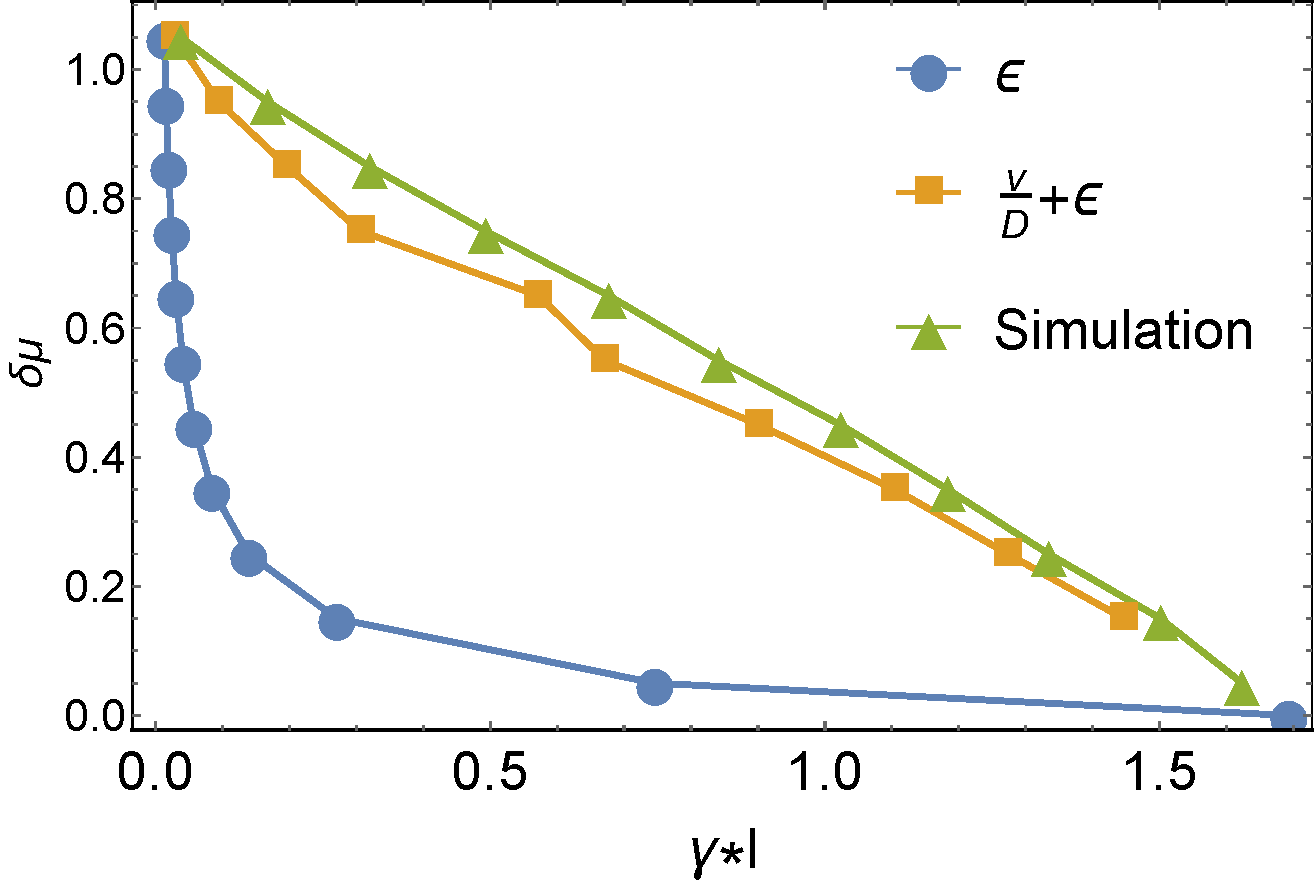
\includegraphics[scale=0.35]{predictepsilonv2.pdf}
\caption{$\delta\mu$ vs. $\gamma$. Instead of predicting the required $\delta\mu$, the blue curve (from Eq. 7) and the orange curve (from Eq. 8) can be used to predict the effective surface tension at certain $\delta \mu$. The data here is for $k_s=4$ and $k_\theta = 6$.} \label{fig:epsilonpredict}
\end{figure}
%P(l_{BE},l_{EC},l_{BC},\widehat{BEC},\widehat{ABE},\widehat{ECD},\widehat{ABC},\widehat{BCD})
% P(l_{BC},\widehat{ABC},\widehat{BCD})
%
%\begin{figure*}
%\centering
%  \subfloat[]{%
%   \includegraphics[scale=0.35]{estimationfordeltamu0d1ver2.pdf}}\hfill
% \subfloat[]{%
%    \includegraphics[scale=0.35]{estimationfordeltamu0d4ver2.pdf}}\\
%  \subfloat[]{
%   \includegraphics[scale=0.35]{estimationfordeltamu0d7ver2.pdf}}\hfill
%  \subfloat[]{%
%    \includegraphics[scale=0.35]{estimationfordeltamu1d0ver2.pdf}}\hfill
%\caption{Comparison of the Fourier Spectrums of the interface's fluctuation at different $\delta\mu$ from simulations and predicted by Eq. 8 in the main text. The data here is for $k_s=4$ and $k_\theta = 6$.} \label{fig:predictandsimulation}
%\end{figure*}


\bibliography{References02232018}
\end{document}